\documentclass[11pt]{report}
\usepackage{fullpage}
%\usepackage{sourcesanspro, sourcecodepro}
\usepackage{minted}
\usepackage{graphicx}
\usepackage{awesomebox}
\usepackage{hyperref}
\usepackage[a4paper, total={6in, 8in}, margin=0.75in]{geometry}
\usepackage{etoolbox}
\makeatletter
\patchcmd{\chapter}{\if@openright\cleardoublepage\else\clearpage\fi}{}{}{}
\RequirePackage[T1]{fontenc}
\RequirePackage[default,light,black]{roboto}

\hypersetup{
    colorlinks=true,
    linkcolor=blue,
    citecolor=blue,
    filecolor=blue,
    urlcolor=blue,
    pdfborder={0 0 0}
}

\graphicspath{{./images/}}

\title{APSC 258: Lab 6 Manual}
\author{Scott Halston}

\begin{document}
\maketitle
\tableofcontents

% page break
\clearpage

\chapter{Introduction}
\section{Introducing Droppout Layers}
In our last lab, you improved your self-driving neural network by introducing convolution layers. Hopefully, in adding convolution layers, you were able to achieve a low training and testing mean squared error (MSE) value. Getting a low training MSE was probably much easier than achieving a low training MSE value. This is because your model became overfit to the training data. To combat this, we will introduce dropout layers in this lab manual.

\section{Overfitting}
Overfitting occurs when a model is trained in a way that produces a model that fits exactly against its training data. When a model is overfitted, the model cannot predict unseen data accurately. Understanding this concept through words is difficult, so below are some graphs to help.

\begin{center}
    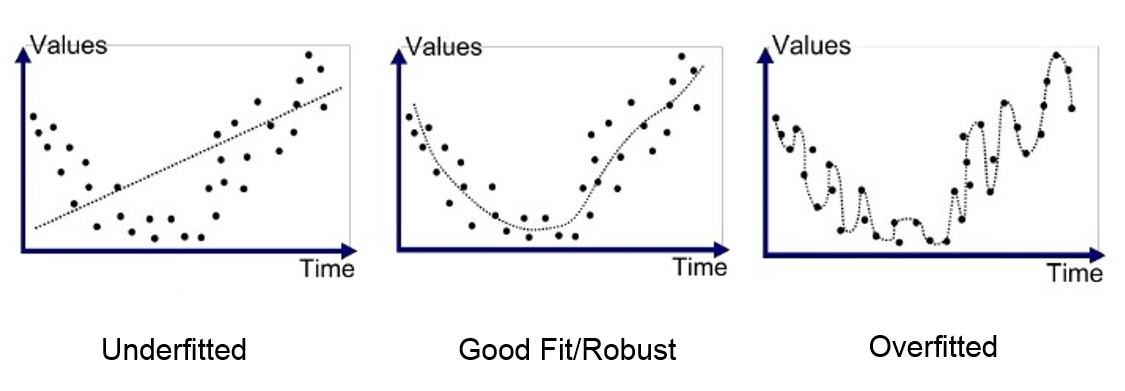
\includegraphics[scale=0.375]{./images/overfitexample.png}
\end{center}

\section{Dropout Layers}
We introduce dropout layers to combat overfitting our models. A dropout layer is a very simple function that randomly drops training data to disrupt the model from becoming overfitted. An example of this can be seen below.

\begin{center}
    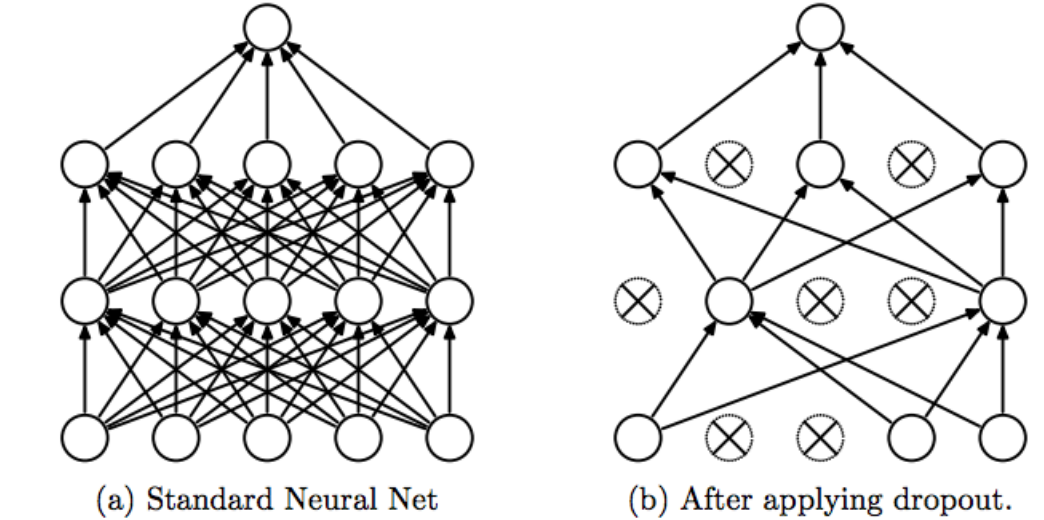
\includegraphics[scale=0.2]{./images/dropoutexample.png}
\end{center}

\chapter{Using Dropout Layers}
Now that we have a better understanding of dropout layers, we can use them in our neural network.


\section{Dropout Layers in Neural Networks}
Below is the same example of a neural network that you saw in the last lab manual; except, this time, it includes dropout layers. For your understanding, all of the parameters are explained within the code. It is highly recommended to go through this code on your own to better your understanding of dropout layers.

\begin{minted}[linenos, fontfamily=courier, style=monokai, bgcolor=black, breaklines]{python} 
    from keras.layers import Conv2D, MaxPooling2D, Dense Sequential, InputLayer, Flatten
    # a sequential model is a model that is made up of layers
    model = Sequential()
    # the input layer is the first layer in the model
    model.add(InputLayer(input_shape=(100, 66, 1)))

    # the convolution layer
    # the different parameters are:
    # the number of output filters: 32
    # the kernel size: (3, 3) specifying the height and width of the 2D convolution window.
    # the activation function: ReLU the type of activation function that is used in the convolution layer.
    model.add(Conv2D(32, kernel_size=(3, 3), activation='relu'))

    # the pooling layer
    # the pooling layer is used to reduce the size of the image.
    # the pool size: (2, 2) specifying the height and width of the 2D pooling window.
    model.add(MaxPooling2D(pool_size=(2, 2)))

    # the dropout layer
    # the dropout layer is used to prevent overfitting the model.
    # increasing or decreasing the value will determine how often the dropout layer randomly drops the training data
    model.add(Dropout(0.1))

    # the flatten layer
    # the flatten layer is used to turn the output of the convolution layer into a 1 dimensional vector.
    model.add(Flatten())

    # our dense layers, used to do the classification
    model.add(Dense(100, activation='relu'))
    model.add(Dense(50, activation='relu'))
    model.add(Dense(10, activation='relu'))
    model.add(Dense(1, activation='relu'))
\end{minted}


\chapter{Applying the Convolution Layer}
Now that you have a good grasp of dropout layers, we can apply it to our own neural network. Open the model that you've been working on over the past 2 labs and add try experimenting by adding dropout layer(s). See if multiple dropout layers function better than a single one and test what values of the dropout layer(s) provide the best results. Once you are happy with your model, you can save the model and download it. You can run the model with the following code.
"python runNetwork.py -m yourConvolutionModel.h5"

\section{Finishing Up}
To complete this lab, you should experiment with dropout layers to achieve both, a low testing and training MSE value.
You now have all of the tools of neural networks available to you to make your model the best it can be! Your next lab manual will detail how your models will be graded and what you should be trying to achieve. For this lab session, try to get the lowest MSE values you can.

\end{document}
